%%%%%%%%%%%%%%%%%%%%%%%%%%%%%%%%%%%%%%%%%%%%%%%%%%%%%%%%%%%%%%%%%%%%%%%%%%%%%%%%
%2345678901234567890123456789012345678901234567890123456789012345678901234567890
%        1         2         3         4         5         6         7         8

\documentclass[letterpaper, 10 pt, conference]{ieeeconf}  % Comment this line out
                                                          % if you need a4paper
%\documentclass[a4paper, 10pt, conference]{ieeeconf}      % Use this line for a4
                                                          % paper

\IEEEoverridecommandlockouts                              % This command is only
                                                          % needed if you want to
                                                          % use the \thanks command
\overrideIEEEmargins
% See the \addtolength command later in the file to balance the column lengths
% on the last page of the document

% The following packages can be found on http:\\www.ctan.org
%\usepackage{graphics} % for pdf, bitmapped graphics files
%\usepackage{epsfig} % for postscript graphics files
%\usepackage{mathptmx} % assumes new font selection scheme installed
%\usepackage{times} % assumes new font selection scheme installed
%\usepackage{amsmath} % assumes amsmath package installed
%\usepackage{amssymb}  % assumes amsmath package installed

\usepackage{graphics} % for pdf, bitmapped graphics files
\usepackage{graphicx}
\usepackage{epsfig} % for postscript graphics files
\usepackage{amsmath} % assumes amsmath package installed
\usepackage{amssymb}  % assumes amsmath package installed
\usepackage{amsfonts}
\usepackage{amsmath} % assumes amsmath package installed
\usepackage{subcaption}
\usepackage{cite}
\usepackage{color}
\usepackage{multirow}
\usepackage{algpseudocode,algorithm,algorithmicx}
%\usepackage[]{algorithm2e}

%\SetKwInput{KwFind}{Find}


\title{\LARGE \bf
Robust Trajectory Planning for a Multirotor Using Funnel Library
}

%\author{ \parbox{3 in}{\centering Huibert Kwakernaak*
%         \thanks{*Use the $\backslash$thanks command to put information here}\\
%         Faculty of Electrical Engineering, Mathematics and Computer Science\\
%         University of Twente\\
%         7500 AE Enschede, The Netherlands\\
%         {\tt\small h.kwakernaak@autsubmit.com}}
%         \hspace*{ 0.5 in}
%         \parbox{3 in}{ \centering Pradeep Misra**
%         \thanks{**The footnote marks may be inserted manually}\\
%        Department of Electrical Engineering \\
%         Wright State University\\
%         Dayton, OH 45435, USA\\
%         {\tt\small pmisra@cs.wright.edu}}
%}

\author{Suseong Kim$^{1}$, Davide Falanga$^{1}$ and Davide Scaramuzza$^{1}$% <-this % stops a space
\thanks{*This work was not supported by any organization}% <-this % stops a space
\thanks{$^{1}$S. Kim is with the Robotics and Perception Group, University of Zurich, Switzerland
        {\tt\small $\{$suseong,falanga,sdavide$\}$ at ifi.uzh.ch}}%
}

\begin{document}

\maketitle
\thispagestyle{empty}
\pagestyle{empty}


%%%%%%%%%%%%%%%%%%%%%%%%%%%%%%%%%%%%%%%%%%%%%%%%%%%%%%%%%%%%%%%%%%%%%%%%%%%%%%%%
\begin{abstract}

This paper is about funnel library that can be used to generate robust trajectories for multirotors.

\end{abstract}


%%%%%%%%%%%%%%%%%%%%%%%%%%%%%%%%%%%%%%%%%%%%%%%%%%%%%%%%%%%%%%%%%%%%%%%%%%%%%%%%
\section{INTRODUCTION}

Throughout the paper, $0_{ij}$ stands for the zero matrix in $\mathbb{R}^{i\times j}$, and $I_i$ denotes the identity matrix in $\mathbb{R}^{i\times i}$. 
For a matrix, $\|\cdot\|$ represents the induced 2 norm, and $\lambda_{\max}(\cdot)$ and $\lambda_{\min}(\cdot)$ indicate the maximum and minimum eigenvalues.
Also, $|\cdot|$ is the Euclidean norm for a vector. 
For two vectors $\alpha,\beta \in \mathbb{R}^{3\times 1}$, 
we denote the inner and cross products as $\langle \alpha,\beta\rangle = \alpha^\top \beta$ and $\textbf{S}(\alpha)\beta = \alpha \times \beta$. 
For two quaternions $\mathbf{q}_1$ and $\mathbf{q}_2$, the quaternion multiplication expressed as $\mathbf{q}_1\otimes\mathbf{q}_2$. 
Also, $\textbf{P}(\cdot)$ is the quaternion representation of a vector $\omega\in\text{so}(3)$ such as $\textbf{P} = [0\;\omega^\top]^\top$. 
The rotation of a vector is indicated as $\mathbf{q}_1\odot\omega = \textbf{q}_1\otimes\textbf{P}(\omega)\otimes\textbf{q}^{-1}$. 
Furthremore, $\text{c}\cdot$ and $\text{s}\cdot$ are shorthands of $\cos\cdot$ and $\sin\cdot$, respectively.

\section{Quadrotor dynamics and control}

\subsection{Quadrotor dynamics}
To describe the dynamic model of a multirotor, we define the inertial $O_I\{x_I,y_I,z_I\}$ and the multirotor body-fixed $O_b\{x_b,y_b,z_b\}$ frames. The body-fixed frame is located at the center of the multirotor. 
The translational and angular dynamics of a multirotor is described as follows:
\begin{align}
\ddot{p} &= gz_I + Tz_b + F_d + \delta \label{eq:translational} \\
\dot{\textbf{q}} &= \textstyle{\frac{1}{2}}\textbf{q}\otimes \text{P}(\omega) \label{eq:rotational}
\end{align}
where $p$ is the position of $O_b$ with respect to $O_I$, and $\textbf{q} = [q_0\;\bar{q}^\top]^\top$ is the unit quaternion describing the orientation of $O_b$ with respect to $O_I$.
The angular velocity of $O_b$ represented in $O_b$ is denoted as $\omega$.
The terms $g$ and $T$ are gravitational constant and mass normalized collective thrust, respectively. 
Without loss of generality, the axis $z_I$ is defined as $e_3 = [0\;0\;1]^\top$.
%Also, the operator $\otimes$ represents quaternion multiplication and $\text{P}(\cdot)$ is the quaternion representation of a vector ${\omega} \in \text{so}(3)$ as $\text{P}({\omega}) = [0\;{\omega}^\top]^\top$. 
The rotor drag applied on the multirotor is denoted as $F_d$, and it is explicitly expressed as follows:
\begin{equation}
F_d = c_d\textbf{q}\odot\pi_z\textbf{q}^{-1}\odot \dot{p} \label{eq:rotorDrag}
\end{equation}
where $c_d$ is the rotor drag coefficient, $\pi_z = I_3 - e_3^\top e_3$ is the matrix projecting a vector onto the $x_by_b$ plane.
%, and the operator $\odot$ denotes quaternion rotation such as $\textbf{q}\odot r = \textbf{q}\otimes\text{P}(r)\otimes\textbf{q}^{-1}$.
The external forces and model uncertainties excluding the rotor drag term are lumped in $\delta \in \mathbb{R}^{3\times 1}$. 

In eq. \eqref{eq:rotational}, angular velocity $\omega$ is used as the input term since the rotational velocity dynamics is fast enough. 
%the rotational motion of a quadrotor is described with the kinematic relation. 
It is possible based on the assumption that the multirotor body angular rate $\omega$ could be directly controlled with low-level controllers such as [DANDREA] or off-the-shelf flight controllers supporting angular rate control mode.
Therefore, the input terms of the multirotor dynamics in eqs. \eqref{eq:translational} and \eqref{eq:rotational} are $T$ and $\omega$.
\\
\textbf{Uncertainty and disturbances}
In the free flight scenario, rotor drag and fuselage drag could be considered as the biggest external disturbances.
The rotor drag could be modeled as, and the fuselage drag could be blah blah.
Non perfect input tracking, XXX

\subsection{Multirotor control} \label{sec:controller}
Let us assume that the reference trajectory of the differential flat output[MEL], which are $\{p(t)^r,\psi^r(t)\}$ and $\mathcal{C}^2$, are given.
Here, $p^r(t)$ is the reference trajectory of the multirotor, and $\psi(t)$ represents the reference rotation of the multirotor about the $z_b$ body axis, i.e. yaw angle in the Euler attitude representation.

To control the translational motion of a multirotor, we utilized a geometric control method [TYL] which is widely utilized in the researches on multirotors [RPG][UPENN][MIT].
Let $e_p = p - p^r$ and $e_v = \dot{p} - \dot{p}^r$ be the position and velocity error terms.
With the above definitions, the mass normalized thrust $T$ and desired thrust direction of a multirotor $z_b^d$ could be computed as the following procedure:
\begin{align}
\ddot{p}^{d} &= -K_p e_p - K_v e_v -ge_3 + \ddot{p}^r \label{eq:ddpd} \\
%z_b^{d} &= \frac{\ddot{x}^{d}}{\|\ddot{x}^{d}\|} \nonumber \\
z_b^{d} &= \ddot{p}^{d}/|\ddot{p}^{d}| \nonumber \\
T &= \langle \ddot{p}^{d}, z_b \rangle = |\ddot{p}^{d}|\langle z_b^d, z_b \rangle \nonumber 
\end{align}
where $K_p$ and $K_v$ are gain matrices with positive diagonal entries.
By substituting the terms $T$ and $\ddot{p}^d$ in \eqref{eq:translational}, the error dynamics of the translational motion could be derived as follows:
\begin{align}
%\dot{e}_p &= e_v \nonumber \\
\ddot{e}_p &= ge_3 + Tz_b + F_d + \delta - \ddot{p}^r + \ddot{p}^d - \ddot{p}^d \nonumber \\
&= -K_pe_p -K_ve_v + F_d + \delta + Tz_b - \ddot{p}^d \nonumber \\
&= -K_pe_p -K_ve_v + F_d + \delta + |\ddot{p}^d|\{\langle z_b^d, z_b \rangle z_b - z_b^d\} \nonumber \\
&= -K_pe_p -K_ve_v + F_d + \delta +  |\ddot{p}^d|\text{s}_\Phi u \label{eq:translationalError1}
\end{align}
%where $\text{s}_\Phi u$ is the term inside of the curly bracket with
where $\Phi$ is the angle between the axes $z_b$ and $z_b^d$, and $u$ is the unit vector indicating the direction of the term inside of the curly bracket.

Similarly, the rotational motion of a multirotor could be analyzed by combining it with a control law that generates the desired angular rate $\omega^d$. 
First, we compute the desired attitude of the multirotor with $\psi(t)$ and $z_b^d$ as follows: [MEL]
\begin{align}
\bar{y}_b &= [\begin{array}{ccc}-\text{s}_{\psi^r}&\text{c}_{\psi^r}&0\end{array}]^\top \nonumber \\
x_b^d &= \text{S}(\bar{y}_b)z_b^d / |\text{S}(\bar{y}_b)z_b^d | \nonumber \\ 
y_b^d &= \text{S}({z}_b^d)x_b^d / |\text{S}(z_b^d)x_b^d |. \nonumber  
\end{align}
Then, based on the axes $\{x_b^d,y_b^d,z_b^d\}$, the desired coordinate could be represented with the unit quaternion $\textbf{q}^d$. 
The attitude error between $\textbf{q}^d$ and $\textbf{q}$ is denoted as $\textbf{q}_e = \textbf{q}^{-1}\otimes \textbf{q}^d$. To decrease the attitude error $\textbf{q}_e = [q_e\;\bar{q}_e^\top]^\top$, the angular velocity is set as 
\begin{equation}
\omega = \left\{
\begin{array}{ll}
\omega_d^d - k_p \bar{q}_e & \text{if  }\;q_e \geq 0, \\ 
\omega_d^d + k_p \bar{q}_e & \text{if  }\;q_e < 0. \\ 
\end{array}
\right.
\end{equation}
where $\omega_d^d$ is the desired angular velocity of $\textbf{q}^d$ represented in $\textbf{q}^d$.
According to [ETH], the attitude error $\textbf{q}_e$ is globally asymptotically stable equilibrium point. 
Hence, it is possible to assume that the error $\Phi$ is also asymptotically stable, and bounded by a known value.
\\
\textbf{Assumption : }
In this work, we assume that the norm of the external disturbance is bounded as $|\delta| \leq \bar{\delta}$. 
Also, the norm of the nominal mass normalized collective thrust value is bounded as $|ge_3 + \ddot{p}^r| \leq \bar{T}$ given any $\mathcal{C}^2$ reference trajectory $x^r$.  
Furthermore, the maximum thrust axis error is bounded such as $\text{s}_\Phi \leq \bar{\text{s}}_\Phi$.

\subsection{Stability analysis}
In Sec. \ref{sec:controller}, it is assumed that the attitude error is bounded for all flight duration.
In this subsection, we investigate the stability of the translational dynamics in eq. \eqref{eq:translationalError1}.  
%could be considered as input-to-state stable by considering $\bar{T}$, $|\dot{p}^r|$, and $\delta$ as input terms. 
As the first step, the dynamics system is summarized as follows: 
\begin{equation}
\begin{array}{l}
\dot{e}_p = e_v \\
\dot{e}_v = -K_pe_p-K_ve_v+F_d+\delta+\text{s}_\Phi|\ddot{p}^d| u. 
\end{array} \label{eq:errorDynamics}
\end{equation}
To analyze the stability of the error dynamics conveniently, we assume that $K_p = k_pI_3$ and $K_v = k_vI_3$ with positive scalar gain values $k_p$ and $k_v$. 
Then, we define the Lyapunov candidate function as $V=\frac{1}{2}e^\top P e$ where $e = [e_p^\top\;e_v^\top]^\top$ and
\begin{equation}
P = \left[
\begin{array}{rr}
(k_p+k_d)I_3 & I_3 \\ I_3 & I_3
\end{array}
\right]. \nonumber
\end{equation}
The Lyapunov function is positive definite when $k_p + k_v > 1$.
Furthermore, the directional derivative of $V$ can be summarized as follows:
\begin{align}
\dot{V} &= -k_p e_p^\top e_p -k_v e_v^\top e_v + e_v^\top e_v \nonumber \\
&\;\;\;\;+(e_p+e_v)^\top\{\delta + F_d + |\ddot{p}^d|\text{s}_\Phi u\}.
\end{align}
Then, by having $\ddot{p}^d$ in eq. \eqref{eq:ddpd}, $|\delta|\leq\bar{\delta}$, $|F_d| \leq c_d|\dot{p}^r+e_v|$, and $|\text{s}_\Phi u| < \bar{\text{s}}_\Phi$, we can rearrange the above relation further as
\begin{align}
\dot{V} &\leq -k_p|e_p|^2 -(k_v+1)|e_v|^2 +(|e_p| + |e_v|)\nonumber \\
&\;\;\;\;\times\{\bar{\delta} + c_d|\dot{p}^r+e_v|+\bar{\text{s}}_\Phi(|-k_pe_p-k_ve_v|+\bar{T})\} \nonumber \\
&\leq -\bar{e}^\top Q\bar{e} + \Delta|\bar{e}| \label{eq:dotV}
\end{align} 
where $\bar{e} = [|e_p|\;|e_v|]^\top$, $\Delta = \bar{\delta}+c_d|\dot{p}^r|+\bar{s}_\Phi\bar{T}$ and
\begin{align}
Q &= \left[
\begin{array}{rr}
k_p(1-\bar{s}_\Phi) & -\frac{1}{2}\{c_d+\bar{s}_\Phi(k_p+k_d)\} \\
-\frac{1}{2}\{c_d+\bar{s}_\Phi(k_p+k_d)\} & k_v(1-\bar{s}_\Phi)-1-c_d
\end{array}
\right].\nonumber 
\end{align}
Here, the matrix $Q$ can be considered as the summation of the two separated parts such as
\begin{equation}
Q = Q_A + \bar{\text{s}}_\Phi Q_B \nonumber
\end{equation}
where
\begin{align}
Q_A &= \left[
\begin{array}{rr}
k_p & -\frac{1}{2}c_d \\ -\frac{1}{2}c_d & k_v-1-c_d
\end{array}
\right] \nonumber \\
Q_B &= \left[
\begin{array}{rr}
-k_p & -\frac{1}{2}(k_p+k_v) \\ -\frac{1}{2}(k_p+k_v) & -k_v
\end{array}
\right].
\end{align}
By setting $k_v > 1+c_d$ and $k_p > \frac{c_d^2}{4(k_v-1-c_d)}$, we can make the matrix $Q_A$ positive definite. 
On the other hand, the matrix $Q_B$ cannot be positive definite since the determinant of $Q_B$ is $\text{det}(Q_B) = -\frac{1}{4}(k_p-k_v)^2 \leq 0$, i.e. $\lambda_{\max}(Q_B)\geq0$ and $\lambda_{\min}(Q_B)\leq 0$.
However, even though $Q_B$ is not positive definite, we can assure that the matrix $Q$ is positive definite with the condition $\bar{\text{s}}_\Phi < -\lambda_{\min}(Q_A)/\lambda_{\min}(Q_B)$
which could readly be achieved since $\bar{\text{s}}_\Phi \approx 0$ with a well designed attitude controller.
Therefore, with the gain values $k_p$ and $k_v$ fulfilling $\lambda(Q) \geq 0$, eq. \eqref{eq:dotV} becomes
\begin{align}
\dot{V} &\leq -\lambda_{\min}(Q)|\bar{e}|^2 + \Delta|\bar{e}| \nonumber \\
&\leq -\lambda_{\min}(Q)(1-\theta)|\bar{e}|^2-\lambda_{\min}(Q)\theta|\bar{e}|^2 + \Delta|\bar{e}| \nonumber
%&\leq -\lambda_{\min}(Q)(1-\theta)|\bar{e}|^2-\lambda_{\min}(Q)\theta|\bar{e}|^2 \nonumber \\
%&\;\;\;\;+ (\bar{\delta}+c_d|\dot{p}^r|+\bar{s}_\Phi\bar{T})|\bar{e}| \nonumber
\end{align}
where $0<\theta<1$. 
%Finally, 
%\begin{equation}
%\dot{V} \leq -\lambda_{\min}(Q)(1-\theta)|\bar{e}|^2,\;\;
%\forall|\bar{e}| \geq 
%\frac{\bar{\delta}+c_d|\dot{p}^r|+\bar{s}_\Phi\bar{T}}{\lambda_{\min}(Q)\theta}. \nonumber
%\end{equation}
%\begin{equation}
%\dot{V} \leq -\lambda_{\min}(Q)(1-\theta)|\bar{e}|^2,\;\;\forall|\bar{e}| \geq L\left[
%\begin{array}{ccc}
%\bar{\delta}&|\dot{p}^r|&\bar{T}
%\end{array}
%\right]^\top
%%\frac{|L|}{\lambda_{\min(Q)}(1-\theta)}. \nonumber
%\end{equation}
%where
%\begin{equation}
%L = \frac{1}{\lambda_{\min}(Q)(1-\theta)}\left[
%\begin{array}{ccc}
%1&c_d&\bar{\text{s}}_\Phi 
%\end{array}
%\right].
%\end{equation}
Therefore, the error dynamics of the translational system of a multirotor is uniformly ultimately bounded. Furthermore, the ultimate bound $b$ could be computed as 
\begin{equation}
b = \sqrt{\frac{\lambda_{\max}(P)}{\lambda_{\min}(P)}\mu^2},\;\;\;
%\mu = \frac{\bar{\delta}+c_d|\dot{p}^r|+\bar{s}_\Phi\bar{T}}{\lambda_{\min}(Q)\theta}. 
\mu = \frac{\Delta}{\lambda_{\min}(Q)\theta}. 
\label{eq:expected}
\end{equation}
% of $\bar{\delta}$, $|\dot{p}^r|$, and $\bar{T}$. In other words, the norm of error is 
%\begin{equation}
%|e| < KL(|e_0|,t-t_0) + K(|[\bar{\delta},|\dot{p}^r|,\bar{T}]|) \nonumber
%\end{equation}
In this analysis, we could know that any error will eventually enter into the ultimate bound $|e| \leq b$ within finite time. 
The ultimate bound is the function of $\Delta$ and it is the combination of $\bar{\delta}$, $|\dot{p}^r|$, and $\bar{\text{s}}_\Phi\bar{T}$. Also, the drag coefficient and the maximum attitude error could be interpreted as the weight terms. 
Hence, the radius of the bound will get bigger by having larger disturbances, reference velocity, and reference acceleration ($\bar{T} = |ge_3 + \ddot{p}^r|$). 
However, even though we could get the general sense on how the error will behave, 
it is difficult to know the tight ultimate bound that the error states actually resides. 
Also, given initial set of error states, it is hard to see how the error evolve before getting into the ultimate bound.

%Keeps converging to the region bound set by the norm of input terms.
%Also, the norm of $L$ is a monotonic function of $c_d$ and $\bar{\text{s}}_\Phi$. 
%%By increasing the attitude error, the norm of $L$ will get larger. 
%%In the same manner, the bigger drag coefficient $c_d$ will grow the norm of $L$.
%Accordingly, the error $|e|$ will be bounded by larger bound with larger values of $\bar{\text{s}}_\Phi$ and $c_d$. 
%%It implies that the trajectory tracking performance will get better by having small drag coefficient and good attitude tracking performance.
%%Finally, the norm of the error $|e|$ will enter the ball with radius $\gamma$ which is $\gamma = \frac{\lambda_{\max}(P)}{\lambda_{\min}(P)}|L|\;|[\bar{\delta}\;\;\bar{T}]|$ [KHALIL].
%%\begin{equation}
%%\gamma = \frac{\lambda_{\max}(P)}{\lambda_{\min}(P)}|L|\;|[\bar{\delta}\;\;\bar{T}]|. \nonumber
%%\end{equation}

\section{Computing funnels}
%Heretofore, the stability of the translational motion of a multirotor has been analyzed. 
%The error $|e|$ will be bounded and the radius of the bound is determined by the norm of disturbance, the norm of the nominal thrust, and the reference velocity. 
%Even though we know how the error would behave and the radius of bound in conservative manner, we cannot find the tight bound of the error state with the above analysis. 
In Sec. \ref{sec:stability}, we checked the general behaviour of the translational error dynamic system in conservative manner.
However, with the funnel analysis with sum of squares optimization tools, we can find the realistic outermost bound on the state $e$.
The concept of funnel and numerical method for computing funnel are mainly adopted from [MAJ]. 
\subsection{Funnel?}
Funnel $\mathcal{F}(t) \subset \mathbb{R}^{6\times 1}$  represents the reachable set of error $e(t)\in \mathbb{R}^{6\times 1}$ given the initial set of error $e(t_0) \in \xi_0$ and a closed-loop dynamic equation.
In other words, the error $e(t_0)$ contained in the set $\xi_0$ will evolve only inside of the set $\mathcal{F}(t)$ for all time.
These property of the funnel could be written as follows:
\begin{equation}
e(t_0) \in \xi_0,\;\xi_0 \subset \mathcal{F}(0)\;\Rightarrow\; e(t) \in \mathcal{F}(t),\;\;\forall t \geq t_0. \label{eq:funnel1}
\end{equation}
%Since the error $e(t_0)$ contained in the set $\xi_0$ will evolve inside of the set $\mathcal{F}(t)$ for alll time, the set $\mathcal{F}(t)$ can be considered as a funnel.

Define a time varying positive definite matrix $P_\mathcal{F}(t) \in \mathbb{R}^{6\times 6}$, a positive parameter $\alpha(t) \in \mathbb{R}$, and $V_\mathcal{F}(t,e) = e(t)^\top P_\mathcal{F}(t) e(t)$.
In the following analysis, $V_\mathcal{F}(t,e)$ will be a Lyapunov function, and $\alpha(t)$ will be the parameter indicating the level of $V_\mathcal{F}(t,e)$.
Then, define a set $\mathcal{F}(t)$ as 
\begin{equation}
\mathcal{F}(t) = \{e(t) \in \mathbb{R}^{6\times 1} | V_\mathcal{F}(t,e) \leq \alpha(t)\} \label{eq:funnel2}
\end{equation}
%Here, for $\hat{e}(t) = \{e|V_\mathcal{F}(t,e) = \alpha(t),\;t\in[t_0,t_f]\}$, let us assume that $V_\mathcal{F}$ and $\alpha$ are constrained such as
%\begin{equation}
%\dot{V}_\mathcal{F}(t,e) < \dot{\alpha}(t)\text{ and }V_\mathcal{F}(t,e) = \alpha(t). \label{eq:funnel3}
%\end{equation}
with $V_\mathcal{F}$ and $\alpha$ constrained such that
\begin{align}
&\dot{V}_\mathcal{F}(t,\hat{e}) < \dot{\alpha}(t), \label{eq:funnel3} \\
&\text{for }\;\;\;\hat{e}(t) = \{e(t)|V_\mathcal{F}(t,e) = \alpha(t),\;t\in[t_0,t_f]\}. \nonumber
\end{align}
%In eq. \eqref{eq:forConstraint}, it is shown that the terms $V_\mathcal{F}$ and $\alpha$ exist.
From the constraint, it is obvious that the state $e(t) \in \mathcal{F}(t)$ cannot escape the sublevel set described by $V_\mathcal{F}(t,e) \leq \alpha(t)$.
Therefore, the set $\mathcal{F}(t)$ defined in eqs. \eqref{eq:funnel2} and \eqref{eq:funnel3}
 complies with the definition of funnel in eq. \eqref{eq:funnel1} [MAJ]. 

Another constraint to fulfill the property of funnel defined in eq. \eqref{eq:funnel1} is related on the initial condition of a funnel. 
At $t = t_0$, the initial set of $e$, i.e. $\xi_0$, should be the subset of $\mathcal{F}(t_0)$. 
%so that we can see how all the error state in $e(t_0) \in \xi_0$ progress as time goes on. 
To satisfy the constraint, we define $\xi_0 = \{e \in \mathbb{R}^{6\times1}|e^\top R e \leq 1\}$ with a positive definite matrix $R$. Then, the constraint can be written as follows:
\begin{equation}
V_\mathcal{F}(t_0,\hat{e}) \leq \alpha(t_0),\;\;\text{for}\;\;\hat{e} = \{e |e^\top R e \leq 1\}.
\end{equation} 

Furthermore, we want to find $V_\mathcal{F}$ and $\alpha$ that represent the tight outer bound of $e$. 
Since $P_\mathcal{F}$ is a positive definite matrix and $V_\mathcal{F}$ is a quadratic function of $e$, 
it is possible to define a ellipsoid that enclosing the level set defined as $V_\mathcal{F}(t,e) = \alpha(t)$.
Then, by minimizing the size of the outer shell, the size of the funnel could be minimized consequently.
The outer ellipsoid can be formulated such as
\begin{align}
&\hat{e}^\top(t) S(t) \hat{e}(t) \leq 1,  \nonumber \\
&\text{ for }\;\;\;\hat{e}(t) = \{e(t)|V_\mathcal{F}(t,e) = \alpha(t),\;t \in [t_0,t_f]\}. \nonumber
\end{align}
where $S(t)\in \mathbb{R}^{6\times 6}$ is the positive definite matrix representing the shape of the outer shell. Note that the volume of the ellipsoid is proportional to the determinant of $S(t)$.

Based on these observations, we can formulate the optimization problem to find the tight funnel surrounding the states $e(t)$ as follows:
\begin{equation}
\begin{array}{rl}
\displaystyle{\inf_{P_\mathcal{F},\alpha,S}} & \int_{t_0}^{t_f} \det{S(t)}\text{d}t \label{eq:optim1} \\
\displaystyle{\text{s.t.}}& \dot{V}_\mathcal{F}(t,\hat{e}) < \dot{\alpha}(t)\text{ for }\hat{e} = \{e(t)|V_\mathcal{F}(t,e) = \alpha(t)\}, \nonumber \\
& \hat{e}^\top S(t) \hat{e} \leq 1\text{ for }\hat{e} = \{e(t)|V_\mathcal{F}(t,e) = \alpha(t)\}, \nonumber \\
%& \xi_0 \subset \mathcal{F}(0,e).
& V_\mathcal{F}(t_0,\hat{e}) \leq \alpha(t_0)\text{ for }\hat{e} = \{e|e^\top R e \leq 1\}. \nonumber
\end{array}
\end{equation}

\subsection{Computing funnel}
We compute the funnels for the multirotor translational error dynamic system.
First of all, 
we define the Lyapunov function in the quadratic form such as $V_\mathcal{F} = e(t)^\top P_\mathcal{F} e(t)$ with the time varying positive definite matrix
\begin{equation}
P_\mathcal{F}(t) = \left[
\begin{array}{cc}
P_p(t) & P_{pv}(t) \\
P_{pv}(t) & P_v(t)
\end{array}
\right] \nonumber
\end{equation}
where $P_p(t)$, $P_{pv}(t)$, and $P_v(t)$ are diagonal matrices with positive entries.
Then, with eq. \eqref{eq:errorDynamics}, the directional derivative of the Lyapunov function $V_\mathcal{F}$ is rearranged as follows: 
\begin{align}
\dot{V}_\mathcal{F} &= -e^\top ( A^\top P_\mathcal{F} + P_\mathcal{F}A) e + e^\top \dot{P}_\mathcal{F}e \nonumber \\
&\;\;\;\;+2e^\top P_\mathcal{F} B(\delta+\text{s}_\Phi|\ddot{p}^d|{u}+F_d) \nonumber
\end{align}
where
\begin{equation}
A = \left[
\begin{array}{rr}
0_{33} & I_3 \\ -K_p & -K_d 
\end{array}
\right],\;\;\;B = \left[
\begin{array}{r}
0_{33} \\ I_3
\end{array}
\right].\nonumber 
\end{equation}
In the right hand side of the above equation, the third term further developed as
\begin{align}
&e^\top P_\mathcal{F} B(\delta+\text{s}_\Phi|-K_p e_p -K_v e_v + ge_3 + \ddot{p}^r|\bar{u}+F_d) \nonumber \\
&\leq |e^\top P_\mathcal{F}B|\{\bar{\delta} + \bar{\text{s}}_\Phi(k_p|e_p| + k_v|e_v| + \bar{T})+c_d|\dot{p}^r+e_v|\} \nonumber \\
%&\leq (p_{pv}|e_p|+p_v|e_v|) \label{eq:normAnalysis} \\
%&\;\;\;\;\times \{\bar{\delta}+\bar{\text{s}}_\Phi(k_p|e_p|+k_v|e_v|+\bar{T})+c_d(|\dot{p}^r|+|e_v|)\} \nonumber
&\leq (p_{pv}|e_p|+p_v|e_v|)\{\bar{\text{s}}_\Phi(k_p|e_p|+k_v|e_v|)+c_d|e_v|+\Delta\} \label{eq:normAnalysis}
\end{align}
where $p_{pv}$, $p_v$, $k_p$, and $k_v$ are maximum eigenvalues of $P_{pv}$, $P_v$, $K_p$, and $K_v$.
Also, $\Delta = \bar{\delta}+c_d|\dot{p}^r| + \bar{\text{s}}_\Phi\bar{T}$.
To handle the error states with the norm $|e_p|$ and $|e_v|$ in eq. \eqref{eq:normAnalysis}, we define two variables $\bar{e}_p\in\mathbb{R}$ and $\bar{e}_v\in\mathbb{R}$ with the following constraints:
%to substitute the terms $|e_p|$ and $|e_v|$ in eq. \eqref{eq:normAnalysis} with the following constraints:
\begin{equation}
\begin{array}{ll}
\bar{e}_p^2 = e_p^\top e_p = |e_p|^2, & \bar{e}_p \geq 0 \\
\bar{e}_v^2 = e_v^\top e_v = |e_v|^2, & \bar{e}_v \geq 0. \\
\end{array} \nonumber 
\end{equation} 
Then, $\dot{V}_\mathcal{F}$ is further developed as follows:
%\begin{align}
%\dot{V}_\mathcal{F} &= -e^\top( P_\mathcal{F}A + A^\top P_\mathcal{F}) e + e^\top \dot{P}_\mathcal{F}e +2(p_{pv}\bar{e}_p+p_v\bar{e}_v) \nonumber \\
% &\;\;\;\times\{\bar{\delta} + \bar{\text{s}}_\Phi(k_p\bar{e}_p+k_v\bar{e}_v + \bar{T})+c_d(|\dot{p}^r|+\bar{e}_v)\} \nonumber \\
%&= -e^\top( P_\mathcal{F}A + A^\top P_\mathcal{F}) e + e^\top \dot{P}_\mathcal{F}e  \label{eq:aaa}\\
% &\;\;\;\;+2(p_{pv}\bar{e}_p+p_v\bar{e}_v)\{\bar{\text{s}}_\Phi(k_p\bar{e}_p+k_v\bar{e}_v) + c_d\bar{e}_v + \Delta\}\nonumber 
%\end{align}
\begin{align}
\dot{V}_\mathcal{F} &\leq -e^\top( P_\mathcal{F}A + A^\top P_\mathcal{F}) e + e^\top \dot{P}_\mathcal{F}e  \label{eq:aaa}\\
 &\;\;\;\;+2(p_{pv}\bar{e}_p+p_v\bar{e}_v)\{\bar{\text{s}}_\Phi(k_p\bar{e}_p+k_v\bar{e}_v) + c_d\bar{e}_v + \Delta\}. \nonumber 
\end{align}

In terms $V_\mathcal{F}$ and $\dot{V}_\mathcal{F}$, the variables of the optimization problem are continuous in $t$. 
However, to make the optimization problem easier to solve, 
we discretized the variables $P_\mathcal{F}$, $\alpha$, and $S$. 
Then, the optimization problem can be reformulated as the following:
\begin{align}
&
\begin{array}{rl}
\displaystyle{\inf_{P_\mathcal{F}(n),\alpha(n),S(n),p_{pv}(n),p_v(n)}} & \displaystyle{\sum_{n=0}^{N}} \det(S(n))  \\
\end{array} \label{eq:optim2} \\
&
\begin{array}{rl}
\displaystyle{\text{s.t.}}& \dot{\alpha}(n) - \dot{V}_\mathcal{F}(n) \geq 0\text{ with constraints $c_1$ to $c_9$},  \\
& 1-e^\top S(n) e \geq 0\text{ with constraints $c_9$ and $c_{10}$}, \nonumber \\
& \alpha(0) - V_\mathcal{F}(0) \geq 0\text{ with constraint $c_{11}$}. \nonumber
\end{array} \nonumber 
\end{align}
where
\begin{equation}
\begin{array}{rlrl}
c_1:& \bar{e}_p^2 = e_p^Te_p,           & c_2:&\bar{e}_p \geq 0 \\
c_3:& \bar{e}_v^2 = e_v^Te_v,           & c_4:&\bar{e}_v \geq 0 \\
c_5:& p_{pv}(n)I_3 \geq P_{pv}(n),      & c_6:&p_{pv}(n)I_3 \geq -P_{pv}(n) \\
c_7:& p_{ v}(n)I_3 \geq P_{ v}(n),      & c_8:&p_{ v}(n)I_3 \geq -P_{ v}(n) \\
c_9:& \alpha(n) - V_\mathcal{F}(n) = 0, & c_{10}:&S(n) > 0 \\
c_{11}:& 1-e^\top R e = 0. &&
\end{array} \nonumber
\end{equation}
The constraints $c_5$ to $c_8$ is added to ensure
% $p_{pv}(n) \geq \lambda_{\max}(P_{pv}(n))$ and $p_v(n) \geq \lambda_{\max}(P_v(n))$ 
 $p_{pv}(n) \geq \|P_{pv}(n)\|$ and $p_v(n) \geq \|P_v(n)\|$ 
with diagonal matrices $P_{pv}(n)$ and $P_v(n)$.
In addition, $\dot{P}_\mathcal{F}(n)$ and $\dot{\alpha}(n)$ could be implemented as
\begin{equation}
\begin{array}{cc}
\dot{P}_\mathcal{F}(n) = \frac{P_\mathcal{F}(n+1) - P_\mathcal{F}(n)}{\text{d}t}, & \dot{\alpha}(n) = \frac{\alpha(n+1)-\alpha(n)}{\text{d}t}. 
\end{array} \nonumber
\end{equation}
The optimization problem in eq. \eqref{eq:optim2} could be transformed into the form of sum-of-squares problem and solved efficiently by referring [MAJ].
\begin{figure*}[t]
\begin{subfigure}[b]{0.5\textwidth}
\centering
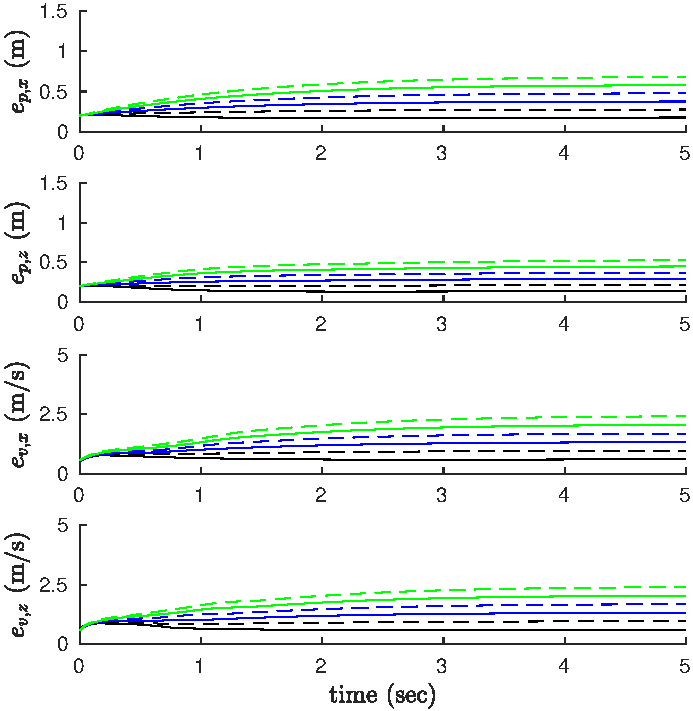
\includegraphics[width=7.0cm]{smaller.pdf}
\caption{Funnels computed with the initial region with $\xi^s$.}
\end{subfigure}
\begin{subfigure}[b]{0.5\textwidth}
\centering
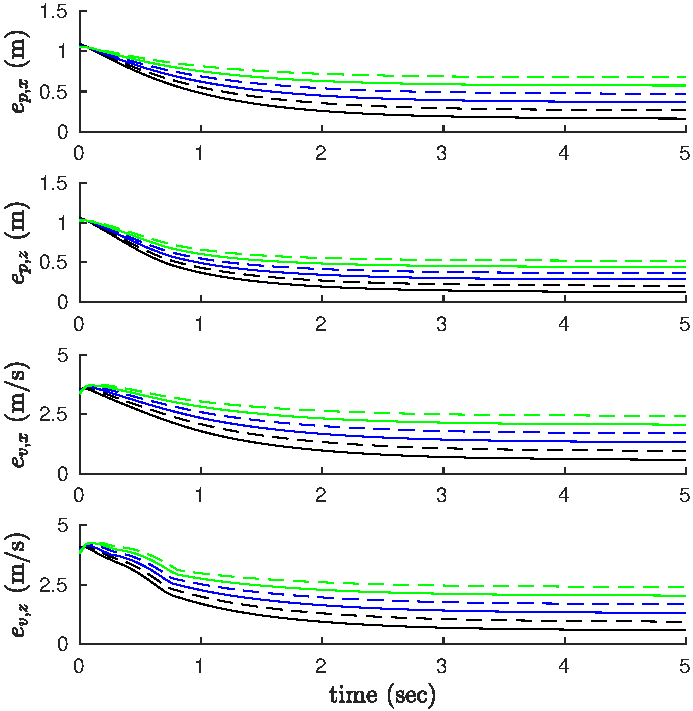
\includegraphics[width=7.0cm]{bigger.pdf}
\caption{Funnels computed with the initial region with $\xi^b$.}
\end{subfigure}
\caption{
Funnels computed with various values of $\Delta_k$ and $\xi_0$. The detailed parameters and settings are available in table. \ref{table:settings}. }
\label{fig:funnelSamples}
\end{figure*}

\subsection{Funnel library}
In the optimization problem, the list of parameters are~: the initial set of error states $\xi_0$; 
the gain matrices $K_p$ and $K_d$; 
the norm of maximum attitude angle error $\bar{\text{s}}_\Phi$;
the rotor drag coefficient $c_d$; and the lumped disturbance term $\Delta$. 
Among these parameters, the gain matrices are manually set by an operator to satisfy the required flight performance in accordance with applications. 
The attitude error $\bar{\text{s}}_\Phi$ and drag coefficient $c_d$ terms should be seleceted to be comparable with respect to the actual values.
Accordingly, the terms $K_p$, $K_d$, $c_d$, and $\bar{\text{s}}_\Phi$ can be set with the current setting of the multirotor.
However, the lumped disturbance term $\Delta(=\bar{\delta}+c_d|\dot{p}^r|+\bar{\text{s}}_\Phi|ge_3 + \ddot{p}^r|)$ keeps changing while a multirotor is in flight. 
For example, the external disturbance, e.g. wind condition, could be different location to location.
Also, the reference velocity $\dot{p}^r$ and accelerations $\ddot{p}^r$ are the function of the reference trajectory so that the terms $|\dot{p}^r|$ and $|ge_3+\ddot{p}^r|$ will change while the multirotor in maneuver.
According to the stability analysis in Sec. \ref{sec:}, 
the radius of the ultimate bound varies with different $\Delta$, 
and the behavior of the error states will also be altered with respect to $\Delta$. 
Therefore, we evaluate \textit{library of funnel} with various values of $\Delta$, and use them depending on the flight condition.
For example, if the external force information is available apriori $\delta$, 
the rest terms $\dot{p}^r$ and $\ddot{p}^r$ are directly computable with the reference trajectory. 
Therefore, before flight operation, we can guess $\Delta$ and look up the library of funnel to see the region that error states can reside while in flight.

Let $\mathcal{B}_\Delta$ be the ultimate bound of the error dynamics when the norm of disturbance is $\Delta$.
For each $\Delta$ value, we evaluate the funnel with two different settings of initial sets $j = \{\xi_s,\xi_b\}$ such that $\mathcal{B}_\Delta\subset\xi_b$ and $\xi_s\subset\mathcal{B}_\Delta$.
By doing this, we can see how the error states behave until they reach their ultimate bound from both smaller and larger regions.

We generate the funnel library with different settings of disturbances $\Delta_l$ with $l(=1,\cdots,L)$ and initial conditions $j=\{b,s\}$ indicating the superscript of $\xi_b$ and $\xi_s$.
Then, a funnel could be denoted as $F_{\Delta_l}^j(n)$ where $n(=1,\cdots,N)$ is the sequence number of funnel generated with the setting $\Delta_l$ and $j$.
In summary, a library of funnel could be organized as the set such as $\mathcal{F} = \{F_{\Delta_1},\cdots,F_{\Delta_L}\}$.
Each element is the funnel $F_{\Delta_l}$ evaluated with different value of disturbance $\Delta_l$, 
and it is constructed with funnels two different set of initial conditions as $F_{\Delta_l} = \{F_{\Delta_l}^b,F_{\Delta_l}^s\}$. The elements are the sequence of compact sets such as $F_{\Delta_l}^j = \{F_{\Delta}^j(0),\cdots,F_{\Delta}^j(N)\}$.
Also, as the definition of the funnel, $F_{\Delta_l}^j(n)$ is the set of of error defined as $P_{\Delta_l}^j(n) \leq \rho_{\Delta_l}^j(n)$ where $P_{\Delta_l}^j(n)$ and $\rho_{\Delta_l}^j$ are the parameters optimzed in the funnel generation.
%$P_{\Delta_l}^j(n)$ and $\rho_{\Delta_l}^j(n)$ are the matrix and values defining an ellipsoid with respect to $F_{\Delta_l}^j(n)$.


As an example, we have generated funnels with the setting in table \ref{table:settings}.
Funnels are optimized with the $\Delta_k$ for every $0.1$ from $0.3$ to $2.5\;[m s^\text{-2}]$. 
The computed funnels are displayed in fig. \ref{fig:funnelSamples}.
The funnel, which is ellipsoid, is projected to each coordinate for visualization purposes.
There are two notable characteristics from the generated funnels shown in fig. \ref{fig:funnelSamples}. 
The first one is that the found ultimate bounds are similar regardless of initial condition if the disturbance $\Delta_k$ is set to similar value. 
The second one is that the ultimate bounds are proportional to the value of $\Delta_k$. 
It is the expected result from the analysis in eq. \eqref{eq:expected}.

\begin{table}[b]
\begin{center}
\begin{tabular}{|r|l||r|l|} 
\hline
param & value & param & value \\ \hline \hline
$\text{d}t$ & 0.05 [s] & $N$ & 120 \\ \hline
$K_{p,x}$ & 10 [s$^\text{-2}$] & $K_{v,x}$ & 4 [s$^\text{-1}$] \\ \hline
$K_{p,y}$ & 10 [s$^\text{-2}$] & $K_{v,y}$ & 4 [s$^\text{-1}$] \\ \hline
$K_{p,z}$ & 15 [s$^\text{-2}$] & $K_{v,z}$ & 6 [s$^\text{-1}$] \\ \hline
\multirow{2}{*}{$\bar{\text{s}}_\Phi$} & 0.035 [$\cdot$] & \multirow{2}{*}{$R^b\;(\xi^b)$} & diag([1.0 1.0 1.0 0.1 0.1 0.1]) \\ 
& $\approx\sin2^\circ$ & & \;\;\;\;\;\;\;\;\;\;\;\;\;\;\;\;\;\;\;\;\;\;\;\;\; [$m^\text{-2}$, $m^\text{-2}s^\text{2}$] \\ \hline
$c_d$ & 0.31 [$s^\text{-1}$]                         & $R^s\;(\xi^s)$ & diag([39 39 39 1.6 1.6 1.6]) \\ \hline
\end{tabular}
\caption{parameters used for computing funnel library} \label{table:settings} 
\end{center}
\end{table}

\subsection{Combining funnels}
\begin{algorithm}
  \caption{Combining funnels around reference trajectory
    \label{alg:funnel}}
  \begin{algorithmic}[1]
    \Statex
    \Function{Combine Funnels }{$\Delta(t)$, $\xi_o$, $\mathcal{F}$}
	\State \textbf{find }$l(0)$\textbf{ s.t.} $\Delta_{l-1} < \Delta(0) \leq \Delta_l$ 
	\State \textbf{find smallest} $F_{\Delta_l} \in {F}$ \textbf{s.t.} ${F}=\{F_{\Delta_l}|\xi_0 \subset F_{\Delta_l}\}$
\State $j(0) \gets $ \text{initial condition of }$F_{\Delta_l}$
\State $n(0) \gets $ \text{index of }$F_{\Delta_l}$
      \For{$t \gets 1 \textrm{ to } T$}
				\State \textbf{find }$l(t)$\textbf{ s.t. }$\Delta_{l-1} < \Delta(t) \leq \Delta_l$
				\If{$l(t) = l(t-1)$}
				\State $j(t) \gets j(t-1)$ 
				\State $n(t) \gets n(t-1)+1$
				\Else
				\State \textbf{find smallest} $F_{\Delta_l} \in {F}$ \textbf{s.t.} 
				\State ${F}=\{F_{\Delta_l}|F_{\Delta_{l(t-1)}}^{j(t-1)}(n(t-1)) \subset F_{\Delta_l}\}$
				\State $j(t) \gets$ \text{initial condition of }$F_{\Delta_l}$ 
				\State $n(t) \gets$ (\text{index of }$F_{\Delta_l}) + 1$
				\EndIf
      \EndFor
      \State \Return{$l(t)$, $j(t)$, $n(t)$}
    \EndFunction
  \end{algorithmic}
\end{algorithm}
Definition of smallest. 
We want to sequence the best fitting funneli, meaning that the ellipsoid with the smallest volume while enclosing the previous funnel.
The volume of an ellipsoid is proportional to the determinant of the matrix $P_{\Delta_l}^j(n)/\rho_{\Delta_l}^j(n)$.
Therefore, we easily can compare the size of the funnels.

How to compute subset?
The center of the ellipsoids are coincident. Then, we can easily check whether $F_1$ is the subset of $F_2$ or not.
Since the sets are defined such as $F_1 = \{e|e^\top R_1 e \leq 1\}$ and $F_2 = \{e|e^\top R_2 e \leq 1\}$, we can show that $F_1 \subset F_2$ is satisfied when $\lambda_{\max}(D_1^{-1}R_2D_1^{-\top} )\leq 1$ where $D_1$ is the Cholesky decomposition of $R_1( = D_1D_1^\top)$.

\subsection{Funnel for checking robustness of reference trajectories}
Once we have a multirotor and a reference trajectory, we can compute funnel around the reference trajectory. 
To check whether the given trajectory robust or not with respect to the obstacles, we can do collision check with the funnel and obstacles.

The method for checking collision between funnel and obstacles will be explained in detail.

%The projected ellipsoid is
%\begin{equation}
%P_x = P_p - P_{pv}^2 P_v^{-1}. \nonumber
%\end{equation}

\section{Simulations}
Monte Carlo simulation will be inserted to show that the funnel can encapsulate the error trajectories as supposed. 
\subsection{Simulation setup}
Simulation setup will be explained. Environment would be the Gazobo integrated with RotorS UAV simulator which explicitely incorporating the rotor drag terms.
Multirotor will follow the minimum snap trajectories generated with to connect randomly generated waypoints.
The initial condition is also randomly generated inside of the ultimate bound. 
Hence, the goal of the simulation is to show that the trajectories starting inside of the ultimate bound (evaluated with the computed funnel) cannot escape the ultimate bound.
\subsection{Simulation results}
Plan is to giving explanation with the following style figure \ref{fig:simulation}
\begin{figure}
\centering
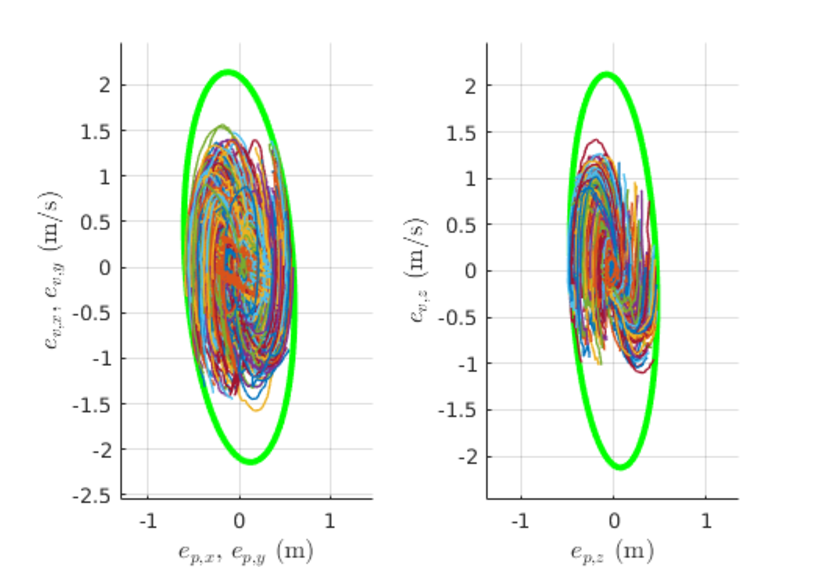
\includegraphics[width=9cm]{monteCarlo.pdf}
\caption{The green ellipse is the ultimate bound projected to each coordinate. 
Since the gains $K_{p,x}$ and $K_{p,y}$, and $K_{v,x}$ and $K_{v,y}$ are set to same values, errors on $x$ and $y$ coordinates are displayed in the same figure.} \label{fig:simulation}
\end{figure}

\section{Experiments}
Experimental scenario is the following. 
We want to find the \textit{safe} velocity that a multirotor can go through a pipe type object as shown in fig. \ref{fig:experimentalResult}.

\subsection{Experimental setup}
\subsection{Experimental results}
\begin{figure*}[!h]
\begin{subfigure}[b]{0.5\textwidth}
\centering
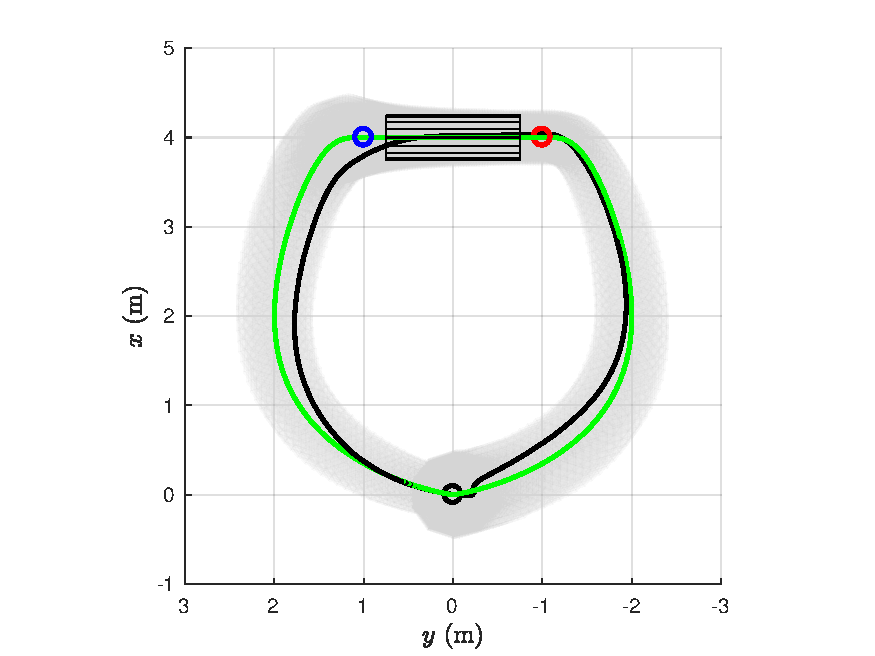
\includegraphics[width=9.0cm]{slow.pdf}
\caption{The reference speed between the blue and red points is $1.0$ m/s.}
\end{subfigure}
\begin{subfigure}[b]{0.5\textwidth}
\centering
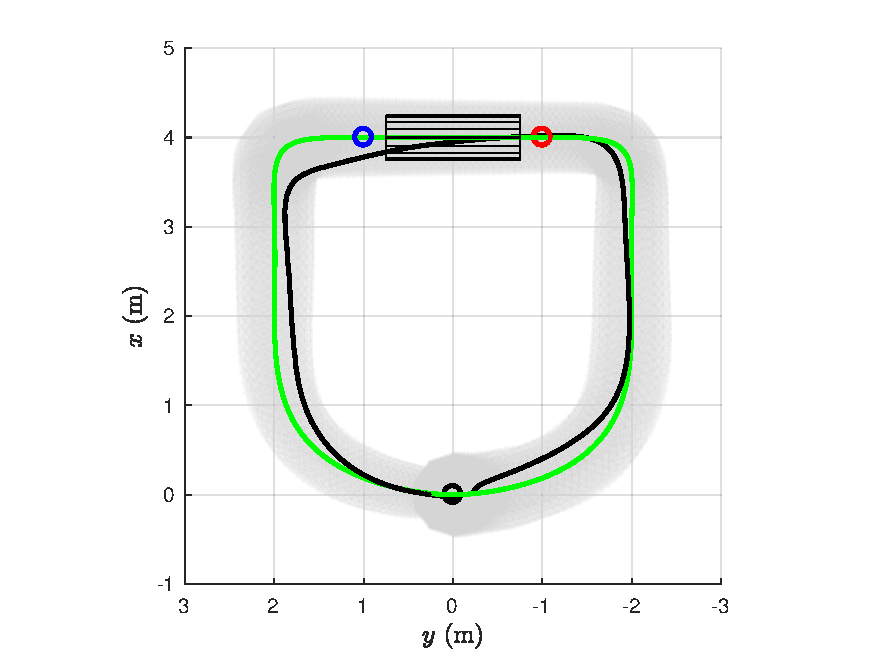
\includegraphics[width=9.0cm]{fast.pdf}
\caption{The reference speed between the blue and red points is $2.6$ m/s.}
\end{subfigure}
\caption{The green and black lines are the reference and measured trajectories, respectively. The shaded regions represent the funnels around the reference trajectory. The goal of this experiment is to move inside of the pipe between the blue and red points safely.}
\label{fig:experimentalResult}
\end{figure*}

\section{CONCLUSIONS}


%\addtolength{\textheight}{-12cm}   % This command serves to balance the column lengths
%                                  % on the last page of the document manually. It shortens
%                                  % the textheight of the last page by a suitable amount.
%                                  % This command does not take effect until the next page
%                                  % so it should come on the page before the last. Make
%                                  % sure that you do not shorten the textheight too much.

%%%%%%%%%%%%%%%%%%%%%%%%%%%%%%%%%%%%%%%%%%%%%%%%%%%%%%%%%%%%%%%%%%%%%%%%%%%%%%%%



%%%%%%%%%%%%%%%%%%%%%%%%%%%%%%%%%%%%%%%%%%%%%%%%%%%%%%%%%%%%%%%%%%%%%%%%%%%%%%%%



%%%%%%%%%%%%%%%%%%%%%%%%%%%%%%%%%%%%%%%%%%%%%%%%%%%%%%%%%%%%%%%%%%%%%%%%%%%%%%%%

\section*{ACKNOWLEDGMENT}


%%%%%%%%%%%%%%%%%%%%%%%%%%%%%%%%%%%%%%%%%%%%%%%%%%%%%%%%%%%%%%%%%%%%%%%%%%%%%%%%


\begin{thebibliography}{99}

\bibitem{c1} G. O. Young, ÒSynthetic structure of industrial plastics (Book style with paper title and editor),Ó 	in Plastics, 2nd ed. vol. 3, J. Peters, Ed.  New York: McGraw-Hill, 1964, pp. 15Ð64.
%\bibitem{c2} W.-K. Chen, Linear Networks and Systems (Book style).	Belmont, CA: Wadsworth, 1993, pp. 123Ð135.
%\bibitem{c3} H. Poor, An Introduction to Signal Detection and Estimation.   New York: Springer-Verlag, 1985, ch. 4.
%\bibitem{c4} B. Smith, ÒAn approach to graphs of linear forms (Unpublished work style),Ó unpublished.
%\bibitem{c5} E. H. Miller, ÒA note on reflector arrays (Periodical styleÑAccepted for publication),Ó IEEE Trans. Antennas Propagat., to be publised.
%\bibitem{c6} J. Wang, ÒFundamentals of erbium-doped fiber amplifiers arrays (Periodical styleÑSubmitted for publication),Ó IEEE J. Quantum Electron., submitted for publication.
%\bibitem{c7} C. J. Kaufman, Rocky Mountain Research Lab., Boulder, CO, private communication, May 1995.
%\bibitem{c8} Y. Yorozu, M. Hirano, K. Oka, and Y. Tagawa, ÒElectron spectroscopy studies on magneto-optical media and plastic substrate interfaces(Translation Journals style),Ó IEEE Transl. J. Magn.Jpn., vol. 2, Aug. 1987, pp. 740Ð741 [Dig. 9th Annu. Conf. Magnetics Japan, 1982, p. 301].
%\bibitem{c9} M. Young, The Techincal Writers Handbook.  Mill Valley, CA: University Science, 1989.
%\bibitem{c10} J. U. Duncombe, ÒInfrared navigationÑPart I: An assessment of feasibility (Periodical style),Ó IEEE Trans. Electron Devices, vol. ED-11, pp. 34Ð39, Jan. 1959.
%\bibitem{c11} S. Chen, B. Mulgrew, and P. M. Grant, ÒA clustering technique for digital communications channel equalization using radial basis function networks,Ó IEEE Trans. Neural Networks, vol. 4, pp. 570Ð578, July 1993.
%\bibitem{c12} R. W. Lucky, ÒAutomatic equalization for digital communication,Ó Bell Syst. Tech. J., vol. 44, no. 4, pp. 547Ð588, Apr. 1965.
%\bibitem{c13} S. P. Bingulac, ÒOn the compatibility of adaptive controllers (Published Conference Proceedings style),Ó in Proc. 4th Annu. Allerton Conf. Circuits and Systems Theory, New York, 1994, pp. 8Ð16.
%\bibitem{c14} G. R. Faulhaber, ÒDesign of service systems with priority reservation,Ó in Conf. Rec. 1995 IEEE Int. Conf. Communications, pp. 3Ð8.
%\bibitem{c15} W. D. Doyle, ÒMagnetization reversal in films with biaxial anisotropy,Ó in 1987 Proc. INTERMAG Conf., pp. 2.2-1Ð2.2-6.
%\bibitem{c16} G. W. Juette and L. E. Zeffanella, ÒRadio noise currents n short sections on bundle conductors (Presented Conference Paper style),Ó presented at the IEEE Summer power Meeting, Dallas, TX, June 22Ð27, 1990, Paper 90 SM 690-0 PWRS.
%\bibitem{c17} J. G. Kreifeldt, ÒAn analysis of surface-detected EMG as an amplitude-modulated noise,Ó presented at the 1989 Int. Conf. Medicine and Biological Engineering, Chicago, IL.
%\bibitem{c18} J. Williams, ÒNarrow-band analyzer (Thesis or Dissertation style),Ó Ph.D. dissertation, Dept. Elect. Eng., Harvard Univ., Cambridge, MA, 1993. 
%\bibitem{c19} N. Kawasaki, ÒParametric study of thermal and chemical nonequilibrium nozzle flow,Ó M.S. thesis, Dept. Electron. Eng., Osaka Univ., Osaka, Japan, 1993.
%\bibitem{c20} J. P. Wilkinson, ÒNonlinear resonant circuit devices (Patent style),Ó U.S. Patent 3 624 12, July 16, 1990. 
%





\end{thebibliography}




\end{document}
